\clearpage
\subsection{Two oxide layers explain a site exchange}
Cut the ideal cell perpendicular to its [001] direction and retain the planes at $z=0$ and $z=\tfrac12$. In one periodically repeated square of the first plane, the four corner contributions sum to one A and the central face contributes one O. In the second plane a central B is surrounded in-plane by four edge oxygens, each shared with an adjacent square, giving one B and two O. Stacking the AO and BO$_2$ layers accounts for one complete formula unit.

\begin{figure}[ht]
\centering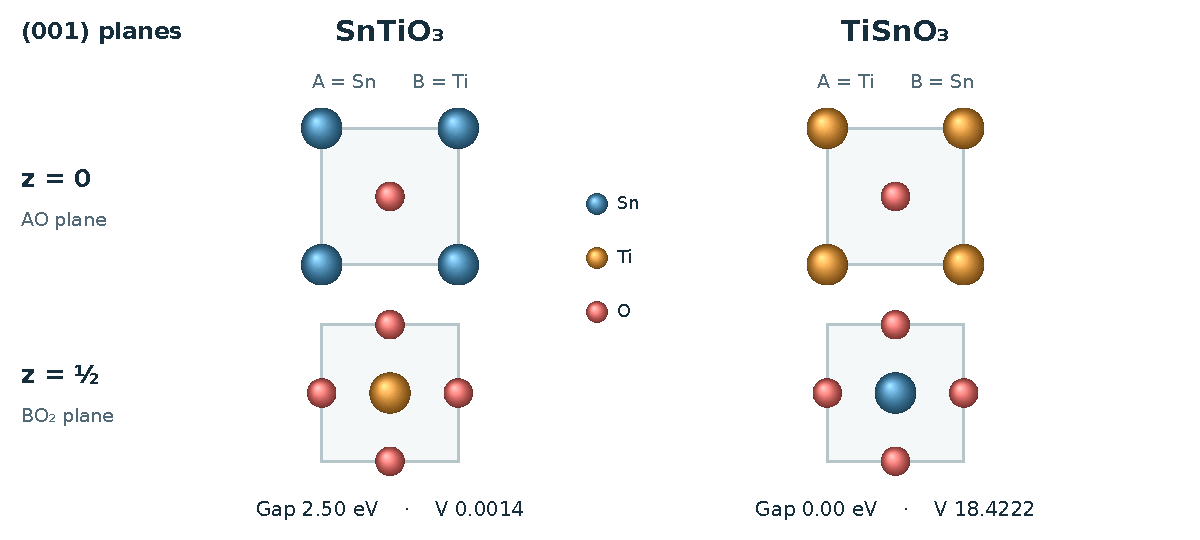
\includegraphics[width=\linewidth]{figures/site_exchange.pdf}
\caption{Equivalent sections through ideal cubic $\mathrm{SnTiO_3}$ and $\mathrm{TiSnO_3}$. Sn is blue, Ti gold and O red throughout. The layer geometry follows the prototype. The gap and violation below each column come from the corresponding public DFT record.}\label{fig:exchange}
\end{figure}

Figure~\ref{fig:exchange} fixes the oxygen framework and exchanges only the cation labels in the idealized drawing. The data describe two separately calculated compositions: their tabulated lattice parameters are 3.969143 and 4.070932~\AA, respectively. The panels use the same fractional coordinates so the two assignments can be compared directly.

Only the CBM threshold is crossed for the first oxide. The resulting loss is $[(4.518833-4.50)/0.5]^2\simeq0.001419$. Under the second assignment the gap collapses to zero, formation energy rises to 1.24 eV, and both band edges take the value 5.758833 eV. The low-gap, formation and CBM terms contribute 7.8400, 4.2436 and 6.3386, respectively. Together they explain the full change to $V=18.422244$. This is a comparison of the supplied labels for two site assignments; attributing the change to a particular orbital interaction would require additional electronic-structure information.

